\documentclass[10pt,a4paper,hidelinks]{report}
\usepackage[utf8]{inputenc}
\usepackage{parskip}
\usepackage{float}
\usepackage[english]{babel}
\usepackage[T1]{fontenc}
\usepackage{lmodern}
\usepackage{xcolor}
\usepackage[left=3cm,
            right=3cm,
            top=2cm,
            bottom=2cm]{geometry}
            
\usepackage{hyperref}
%%%%%%%%%%%%%%% Colors %%%%%%%%%%%%%%%
\usepackage{xcolor}
\usepackage{sectsty}
\definecolor{fib_red}{RGB}{191,21,64}
\definecolor{fib_gray}{RGB}{111,111,111}
\definecolor{blue_upc}{RGB}{52,120,186}
\definecolor{dark_green}{rgb}{0.0, 0.4, 0.0}
\subsectionfont{\color{fib_red}}
\subsubsectionfont{\color{fib_gray}}
\renewcommand\fbox{\fcolorbox{black}{fib_red!20}}

\usepackage{booktabs}
\usepackage{verbatim}
\newcommand{\colorverb}[2]{\textcolor{#1}{\texttt{\detokenize{#2}}}}
\newcommand{\type}[1]{\colorverb{dark_green}{#1}}
\newcommand{\code}[1]{\colorverb{dark_green}{#1}}

\usepackage{caption}
\usepackage{subcaption}

\usepackage{listings}
\lstdefinestyle{mystyle}{
  backgroundcolor=\color{gray!10},
  stringstyle=\color{green!50!black},
  keywordstyle=\color{fib_red},
  numberstyle=\tiny\color{fib_gray},
  commentstyle=\color{blue_upc},
  basicstyle=\ttfamily\footnotesize,
  breakatwhitespace=false,         
  breaklines=true,                 
  captionpos=b,                    
  keepspaces=true,                 
  numbers=left,                    
  numbersep=5pt,                  
  showspaces=false,                
  showstringspaces=false,
  showtabs=false,                  
  tabsize=2
}

\lstset{style=mystyle}


\usepackage{fancyhdr}
\fancyfoot[R]{\raisebox{-0.5\baselineskip}{
\includegraphics[scale=0.25]{assets/images/upc_logo.jpeg}}}
\fancyhead[L]{}
\usepackage[Bjornstrup]{fncychap}

\usepackage{etoolbox}
\makeatletter
\patchcmd{\@makechapterhead}{50\p@}{0\p@}{}{}
\patchcmd{\@makeschapterhead}{50\p@}{0\p@}{}{}
\makeatother

\usepackage{background}

\newcommand{\documentStatus}{SUBMITTED}

\newcommand{\subtitle}[1]{
    \posttitle{
    \par\end{center}
    \begin{center}\Large\bfseries#1\end{center}
    }
}

\setcounter{tocdepth}{1}


\begin{document}
\pagestyle{plain}
\backgroundsetup{contents=,color=red!30}
\pagecolor{white}

% \begin{center}
%     \color{red!50!white}
%     \textbf{\huge{STATUT - \documentStatus}}
% \end{center}

\vfill

\color{black}
\begin{center}
    % \includegraphics[width=0.5\linewidth]{images/logos/fib.png} \\
    
\includegraphics[height=2cm]{assets/images/upc_logo.jpeg} \\
    \vfill
    \rule{\linewidth}{0.5mm} \\[1cm]
    {\Huge \textsc{\textcolor{fib_red}{ML Project}}}\\[0.5cm]
    {\Large \textsc{\textbf{Machine Learning Analysis of Train stations}}}\\[1cm]
    {\Large \textsc{Assignment}}\\[0.4cm]
    {\huge \textsc{\textbf{Machine Learning}}}\\[1cm]
    {\large \textsc{Master in Research and Innovation - UPC\\Master in Data Science, UPC}}\\[0.4cm]
    \rule{\linewidth}{0.5mm} \\[1.5cm]
\end{center}

\vfill

\textbf{Authors :}
\begin{itemize}
    \item Julie \textsc{Oppedal}\newline
    \textit{(Civil Engineering student at University of Bergen, Exchange Student at UPC)}
    \item Pierre \textsc{Jézégou}\newline
    \textit{(Engineering student at École Centrale de Lille, Exchange student at UPC)}
\end{itemize}

\newpage
\color{black}
\pagecolor{white}
\pagestyle{fancy}
\tableofcontents
\section*{Introduction \& Context}
Understanding how many passengers use train stations and what features they have is important for improving transportation services. We're using machine learning to analyze train station data and predict passenger traffic.

To start, we're gathering data from reliable sources like the SNCF and INSEE websites to create a detailed dataset with lots of information about cities and train stations.

Next, we're cleaning up the data to fix errors and make sure it's good for analysis. Then, we'll use different machine learning models to try and figure out the best way to predict passenger traffic and understand what factors make some stations busier than others.

Overall, this project focuses on using advanced computer techniques to optimize transportation services by accurately predicting passenger traffic and understanding station dynamics.

All the code is available in this repository
\begin{center}
    \textcolor{fib_red}{\url{https://github.com/pierre-jezegou/fib-ml-project}}
\end{center}
\chapter{Build and understand dataset}
First and foremost, we have to build a coherent dataset (by cross-referencing sources) to be able to train the models depending on what information are available and how do we want to use it. A wealth of data is available on the "SNCF" and "INSEE" websites: the company and the organization make available a vast amount of open data \url{https://ressources.data.sncf.com}, \url{https://statistiques-locales.insee.fr/}.

\section{Build dataset}
Deliverable of this chapter: The built dataset (before preprocessing) is available on on GitHub:
\begin{center}
    \url{https://github.com/pierre-jezegou/fib-ml-project/releases/download/build-dataset-1.0.3/dataset.csv}
\end{center}
This construction allows us to have enough data (especially features), from two different and independent sources, to obtain an analysis as close as possible to reality. All the raw csv files are stored in the \code{data/} folder in the repository.

\subsection{Consolidating City Statistics and Attraction Area Data (INSEE)}
In \href{https://github.com/pierre-jezegou/fib-ml-project/blob/main/consolidate_cities.py}{\code{consolidate_cities.py}} the process of consolidating city statistics and attraction area data is described. This involves loading, cleaning, merging, aggregating, translating column names, and exporting the consolidated dataset.

The process starts by loading two datasets from INSEE institute, \code{cities_statistics.csv} and \code{attraction_area_per_city.csv}, containing city statistics and information on attraction areas, respectively. After merging the datasets based on \code{city_code}, the numeric data is aggregated per \code{Aire d'attraction des villes 2020} to obtain summarized statistics for each attraction area. Column names are translated to English for clarity and consistency, and the consolidated dataset is exported as \code{consolidated-cities.csv} for further analysis.

\subsection{Building Train Station Dataset (SNCF) - Final dataset}
Then, the process of constructing a dataset related to train stations is done in several steps of data transformation, merging, and integration with cities information.

\subsubsection{Data Transformation}
First, we need to improve columns' data coherence between files: \code{transform_uid} function is defined to format the UIC code into a standardized string format. Then, raw datasets provided by SNCF are processed:
\begin{itemize}
    \item \code{frequentation-gares-raw.csv}: This dataset, representing train station traffic, undergoes transformation where the 'UIC' column is converted to string format and filled to a length of 10 characters with leading zeros. Additionally, the column 'Nom de la gare' is renamed to 'Gare' for clarity.
    \item Other datasets such as services in stations \code{gares-equipees-du-wifi-raw.csv}: be sure to have a clear UIC code to allow merging operations.
\end{itemize}

\subsubsection{Data Merging}
The datasets are then merged using the \code{merge_data_train_stations} function: it iterates through a list of file names, merges datasets based on the 'UIC' column, and performs necessary column operations for clarity.

\subsubsection{Integration with Consolidated Cities}
The resulting train station dataset is then integrated with consolidated cities information. The dataset containing consolidated cities data is loaded, and a merge operation is performed based on the \code{city_code} column. The final merged dataset is saved as \code{dataset.csv}.

\begin{lstlisting}[language=Python]
result = pd.merge(train_stations, consolidated_cities, on="city_code")
\end{lstlisting}

The final columns (features) are describe in the README file in the GitHub repository: \url{https://github.com/pierre-jezegou/fib-ml-project/blob/main/README.md}

\section{Dataset inspection}
\subsection{First inspection}
First, we analyzed the dataset using the \code{dataset.describe()} function from pandas. Our interpretations are as follows:
\begin{itemize}
    \item \textbf{Zero Values}: Some numerical columns, such as \code{total_passengers_2022}, have suspicious zero values needing special handling.
    \item \textbf{High Variability}: Columns like \code{total_passengers_2022} exhibit high standard deviations, indicating significant variability.
    \item \textbf{Missing Data}: Columns such as \code{distr_histoires_courtes} have significantly fewer entries, indicating missing data that may require imputation or removal.
\end{itemize}
Next steps include handling missing values by imputing or removing them, normalizing or standardizing numerical columns for machine learning models, and identifying and handling outliers to ensure robust analysis.\\

We can also have check how many missing values do we have on each variable: \code{dataset.isna().sum()}. For some of the train station related features, there are 7 missing values, but for services provided in stations, there are lot more missing data : 2179. We have to take a decision regarding those two types of missing values.

\subsection{Understand the data}
\begin{figure}[h]
    \centering
    \begin{subfigure}[b]{0.45\textwidth}
         \centering
         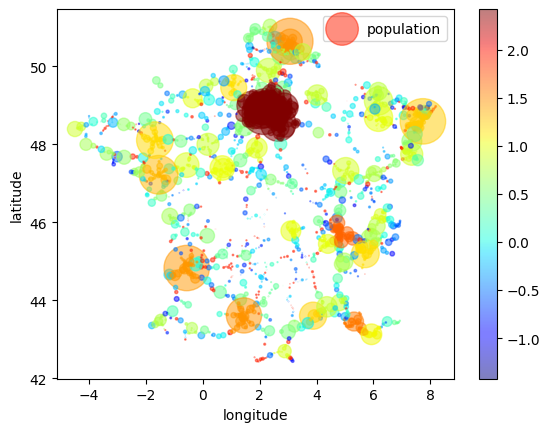
\includegraphics[width=\textwidth]{assets/images/french-map-train-stations.png}
     \end{subfigure}
    \hfill
     \begin{subfigure}[b]{0.4\textwidth}
         \centering
         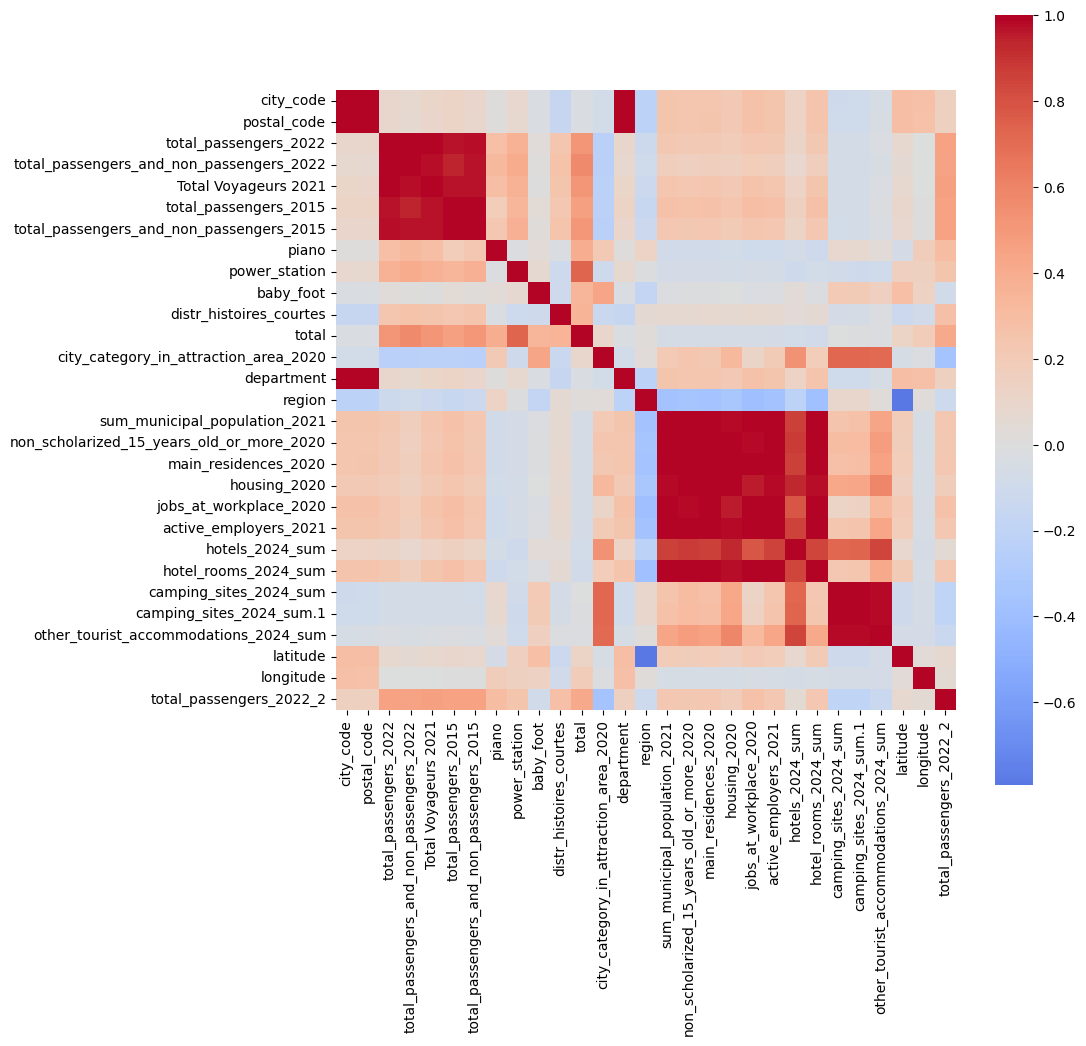
\includegraphics[width=\textwidth]{assets/images/variable-correlation.png}
     \end{subfigure}
     \caption{Examples of data visualizations to understand the dataset}
\end{figure}
Since Paris is the hub for many train lines, we think it can be interesting to compute the distance to Paris. We also observed strong correlations between some variables, so we will remove redundant ones during feature engineering.\label{paris:center-france}
\chapter{Preprocessing}

\section{Deal with missing values}
\subsection{Too many missing values}
Lets have a look on some precise columns where we suppose that there is not enough data. We can use pandas functions.
\begin{lstlisting}[language=python]
>>> dataset.piano.value_counts(dropna=False)
piano
NaN    2179
1.0      48
0.0      28
2.0       1
Name: count, dtype: int64
\end{lstlisting}
And this is the same problem with the majority of the services provided in the train stations, such as \code{power_station}, \code{baby_foot}, \code{distr_histoires_courtes}, \code{total}. This can be analysed as followed: no surveys were organized in those small train station. We could consequently fill all the cells with \code{0} value. But this can bias the final result. We finally decided to drop all these columns because we decided that it was directly correlated with how many people are using this station (sort of return on investment made by SNCF).

\subsection{Some missing values}
Then, we can focus, with almost the same method to other columns.
\begin{lstlisting}[language=python]
>>> (dataRead.total_passengers_2022	==0).value_counts()
total_passengers_2022
False    2246
True       10
Name: count, dtype: int64
\end{lstlisting}
We can see that there are 10 rows containing always 0 value for all the fields. This happen when a city is mentionned 2 times for 2 different trains (for example high speed trains and high speed trains from airport). We chose to remove those lines because passengers has already been counted once.
\begin{lstlisting}[language=python]
dataRead=  dataRead[(dataRead.total_passengers_2022!=0)
            & (dataRead.total_passengers_and_non_passengers_2022!=0) 
            & (dataRead.total_passengers_2015!=0)
            & (dataRead.total_passengers_and_non_passengers_2015!=0)
            ]
dataRead.shape
\end{lstlisting}
Then, we identified that the \code{wifi_service} column contains the values \textit{'Non'} (No), \textit{'Oui'} (Yes), and some missing values (NaN). The distribution of these values was as follows:
\begin{lstlisting}[language=python]
>>> dataset.wifi_service.value_counts(dropna=False)
wifi_service
Non    2106
Oui     120
NaN      8
Name: count, dtype: int64
\end{lstlisting}
To handle the missing values and convert the categorical values to binary, we: We removed rows with \code{NaN} values in the \code{wifi_service column} and converted \code{"Oui"} to 1 and \code{"Non"} to 0. We encountered duplicates for the same train station, missing values for WiFi, and other missing numerical values.

\section{Outliers}
As we have a look at the outliers, we notice there are a significant amount in the following columns: (\code{total_passengers_2022}), (\code{total_passengers_and_non_passangers_2022}), (\code{total_passengers_2015}), and (\code{total_passengers_and_non_passangers_2015}). We have decided to keep these as they are directly relevant to the prediction on how many people a train station is likely to generate. 

There were some outliers for other columns as well, but not a significant amount. Therefore we decided to keep them as well.


\section{Feature extraction}
We did a lot of feature engineering and researches to find the most relevant features to add to our dataset.
\begin{itemize}
    \item Evolution rate between 7 years: we found interesting to compute the evolution rate in term of passengers in the train station between two different years in the past. Indeed, some improvements (such as new train lines, infrastructure changes, construction work...) have been done in train stations leading to an increase of passengers in the train stations. As a consequence, it is directly linked to our topic.
    \item Split geographical coordinates into latitude and longitude. To allow a better comprehension of the dataset and be able to plot geographical dependant figures.
    \item Distance to Paris (country city center). As explained in \ref{paris:center-france}, we chose to compute the distance to the main city.
    \item From numerical value to categories: to be able to use categorical data in models which are just accepting numerical values, we mostly chose to use \href{https://scikit-learn.org/stable/modules/generated/sklearn.preprocessing.OneHotEncoder.html#sklearn.preprocessing.OneHotEncoder}{One hot encoder}. It means creating as much binary columns as there are categories in a given column.
\end{itemize}


\section{Gaussianity, transformations and normalization}
To prepare the data for machine learning models, it is important to ensure the features are on a similar scale and follow a Gaussian distribution where possible. We applied the following transformations:
\begin{itemize}
    \item \textbf{Normalization:} Numerical columns were normalized using the StandardScaler from sklearn.
    \item \textbf{Log Transformation:} For skewed data, we applied log transformation to approximate Gaussianity.
\end{itemize}
\begin{lstlisting}[language=python]
from sklearn.preprocessing import StandardScaler
scaler = StandardScaler()
numerical_cols = ['total_passengers_2022', 'total_passengers_and_non_passengers_2022', 'total_passengers_2015', 'total_passengers_and_non_passengers_2015']
dataset[numerical_cols] = scaler.fit_transform(dataset[numerical_cols])
\end{lstlisting}


\section{Feature selection}
\subsection{Correlation between variables}
We removed over-correlated variables to reduce redundancy and avoid multicollinearity in our model.

\subsection{Non relevant features}
We removed features that did not add significant value to the model.

\section{Helper functions}
To simplify the workflow, we developed different auxiliary functions:
\begin{itemize}
    \item Distance to Paris: we used the \textit{as the crow flies} distance. You can find the implementation in the \href{https://github.com/pierre-jezegou/fib-ml-project/blob/main/distance_calculation.py}{\code{distance_calculation.py}}.
    \item Export metrics to compare models: we wanted to retrieve all the metrics in one single file to be able to compare as easily as possible the models (\code{write_metrics_in_csv})
    \item Plot the variable importance: as we use for each model the variable importance, we decided to implement it one time and use in all our notebooks: \code{plot_variable_importance}
    \item Other functions were implemented to make our lives easier: \code{plot_ypred_vs_yreal} (to compare predictions with real values, with log axis or not...), \code{learning_curve_plot}...
\end{itemize}


\section{Resampling protocols}
As presented in the dataset inspection, our dataset is not very well balanced regarding the target value (passengers). Indeed, there are not a lot of train stations with a lot of passengers: some of the main train stations just aggregate most of the traffic (in term of quantity of passengers). As a consequence, we have very few data for high traffic stations and the models will be influenced maily by the little train stations (whereas the main ones have to be very influent).

\subsection{Potential issues}
This means that when we want to scale up (i.e. generalize the model), we may run into major difficulties. Indeed, new data concerning large stations can have a fairly significant impact on model data. Even if methods exist to overcome these problems, we need to be vigilant.

\subsection{Oversampling or undersampling}
First, we could not do undersampling to remove some of the little stations. Indeed, we don't have so much data to accept removing 1/3 of our data (for example). Then, it is impossible to collect more data (there is no additional data available). So the solution could be to use oversampling methods.
\subsection{SMOTE}
We chose to use SMOTE algorithm for our regression problem to create more points regarding low-traffic train stations as if we wanted to deal with class imbalance in a classification problem. The problem was there were too few points (and the points were too spread out to be able to use this method.
\begin{lstlisting}[language=Python]
# SMOTE
smote = SMOTE(random_state=42)
X_resampled, y_resampled = smote.fit_resample(X, y)
\end{lstlisting}
\begin{lstlisting}
ValueError: Expected n_neighbors <= n_samples_fit, but n_neighbors = 6, n_samples_fit = 1, n_samples = 1
\end{lstlisting}

\subsection{Synthesize data}
As SMOTE was impossible to use due to lack of data points in high-traffic stations, we tried to generate new data points copying points. We also chose to add some noise to add more realism to the new generated points. In the end, it didn't prove very useful in terms of performance. These steps will therefore not be retained in the main preprocessing script (but in this file)\\

You can find all what we implemented for these parts in the following notebook:\\
\href{https://github.com/pierre-jezegou/fib-ml-project/blob/main/models/sampling.ipynb}{\code{models/sampling.ipynb}}


\chapter{Models implementation}
\section{Linear, ridge and lasso regression}
In this chapter, we implemented linear models: linear regression and ridge regression.
\subsection{Final preprocessing}
Before fitting the linear regression model, it is crucial to preprocess the data. As a consequence, we use the preprocessed dataset prepared earlier.
First and foremost, we have to prepare the sets. We have first to separate the features columns from the target. Then, we split the data into 2 subsets: one for the training and one for the test. We will use later cross-validation on the train dataset.
\begin{lstlisting}[language=python]
X = dataset.loc[:,dataset.columns != 'total_passengers_2022']
y = dataset['total_passengers_2022']
X_train, X_test, y_train, y_test = train_test_split(X, y, test_size=0.33, random_state=42)
\end{lstlisting}

\subsection{Model Implementation and Justification}
The implementation of the linear regression model can be efficiently handled using the \code{scikit-learn} library. The \code{Pipeline} and \code{ColumnTransformer} classes facilitate seamless preprocessing and model training.

\subsubsection{Pipeline and ColumnTransformer}
As the linear regression model only require numerical fields, we need a final preprocessing step to convert any categorical data to numerical one. We chose to use \href{https://scikit-learn.org/stable/modules/generated/sklearn.preprocessing.OneHotEncoder.html}{One Hot Encoder} to convert a $m$-categorical feature into $m$ binary feature.
The \code{ColumnTransformer} allows us to apply different preprocessing steps to numerical and categorical features within a single pipeline. This modularity ensures that each type of data receives the appropriate transformations.

\begin{lstlisting}[language=Python]
preprocessor = ColumnTransformer(
    transformers=[
        ('num', StandardScaler(), num_features),
        ('cat', OneHotEncoder(), cat_features)
    ])
\end{lstlisting}

We use the \code{Pipeline} class to chain the preprocessing steps and the linear regression model. This approach enhances code readability and reproducibility.
\begin{lstlisting}
model = Pipeline(steps=[
    ('preprocessor', preprocessor),
    ('regressor', <MODEL>())
])
\end{lstlisting}

This strategy will be used in the following models because it added a more comprehensive way to define a model and simplifies the encoder. We firstly implemented the one hot encoder in the preprocessing part, but we finally moved the steps in each model to be able to test with or without it.

We first implemented very simple model without , just using Scikit Learn \code{LinearRegression} models. To make our model more robust, we then chose to use \textit{Ridge regularization} (to bound the complexity) and cross-validation. We also implement our own model to practice linear algebra manipulation with Python, but we chose to not include in the model comparison.

\subsection{Ridge and Cross validation}
\begin{itemize}
    \item Ridge regression is a regularization technique. It modifies the ordinary least squares method by adding a penalty to the regression coefficients.
    \item We used cross-validation to ensure our linear regression model's results are robust and reliable. This technique helps prevent overfitting by verifying that the model performs consistently across different subsets of the data, providing a more accurate estimate of its generalizability to new, unseen data.
\end{itemize}
The \href{https://scikit-learn.org/stable/modules/generated/sklearn.linear_model.Ridge.html}{documentation} propose several parameters in addition to $\alpha$. For the cross validation, we chose to use directly \code{GridSearchCV} instead of writing imbrication of \code{for} loops to get the best parameters.
\begin{lstlisting}[language=Python]
param_grid = { 'regressor__alpha': [0.1, 1, 10, 100], ...}
grid_search = GridSearchCV(estimator=model, param_grid=param_grid, cv=5)
\end{lstlisting}

\subsection{Results}
We use the helper functions defined in the first chapter to plot some pictures to analyse the perfromances of our model.

\subsubsection{Raw results}
\begin{table}[h]
    \centering
    \begin{tabular}{ccccc}
        \toprule
        Model &  MSE &  MAE & MedianAE & $R^2$ Score \\
        \midrule
        Linear reg. & 4.232e+10 & 54041 & 20135 & 0.968842\\
        Ridge + CV & 4.242e+10 & 51118 & 15273 & 0.968726\\
        Lasso + CV & 4.366e+10 & 52531 & 15043 & 0.967857\\
        \bottomrule
    \end{tabular}
    \caption{Main metrics to compare linear models}
\end{table}
\begin{figure}[h]
    \centering
    \begin{subfigure}[b]{0.3\textwidth}
         \centering
         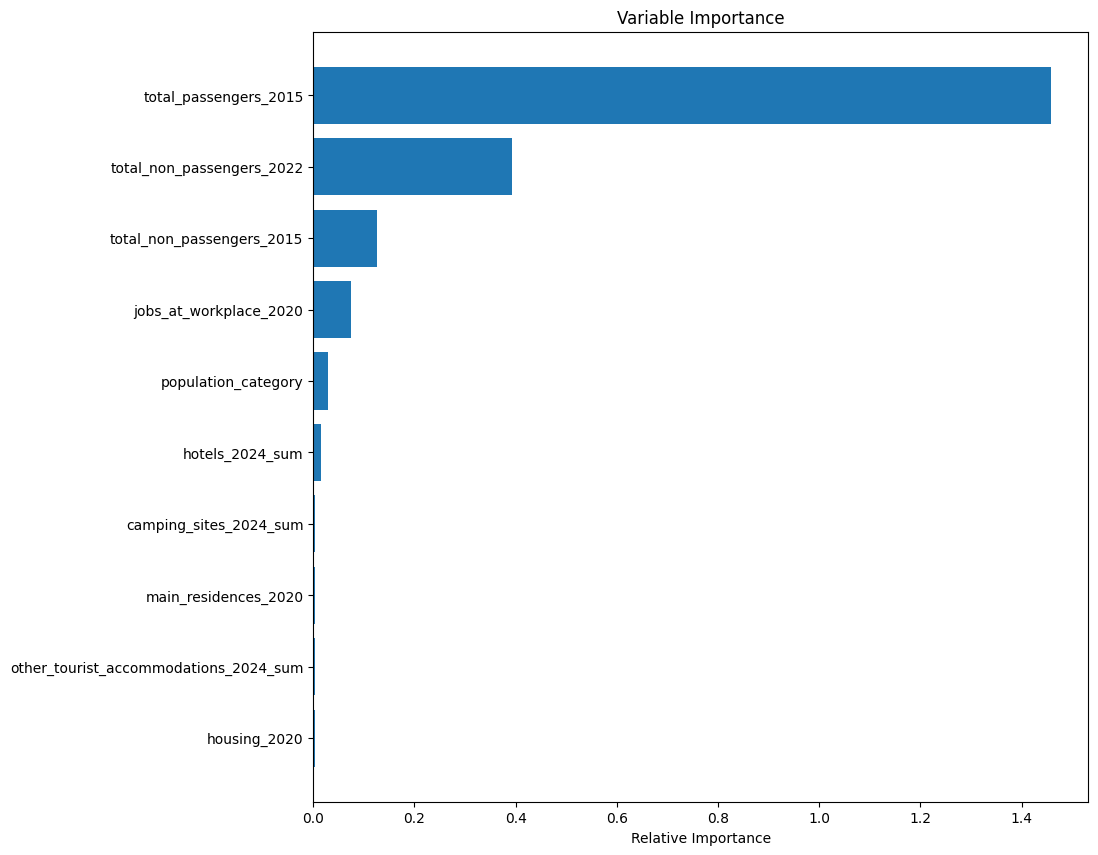
\includegraphics[width=\textwidth]{assets/images/feature-importance-lasso.png}
         \caption{Lasso: Feature importance}
     \end{subfigure}
    \hfill
     \begin{subfigure}[b]{0.3\textwidth}
         \centering
         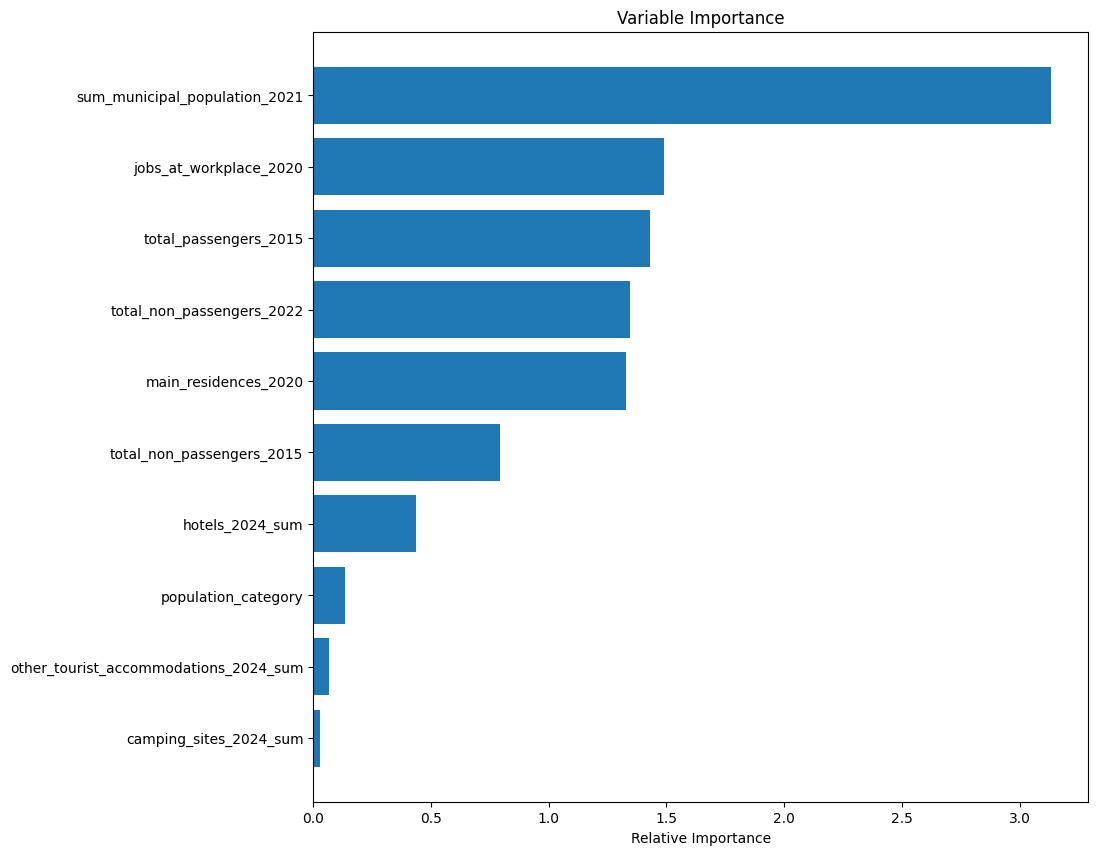
\includegraphics[width=\textwidth]{assets/images/simple-linear-regression-feature-importance.png}
         \caption{Ridge: Feature importance}
     \end{subfigure}
     \hfill
     \begin{subfigure}[b]{0.3\textwidth}
         \centering
         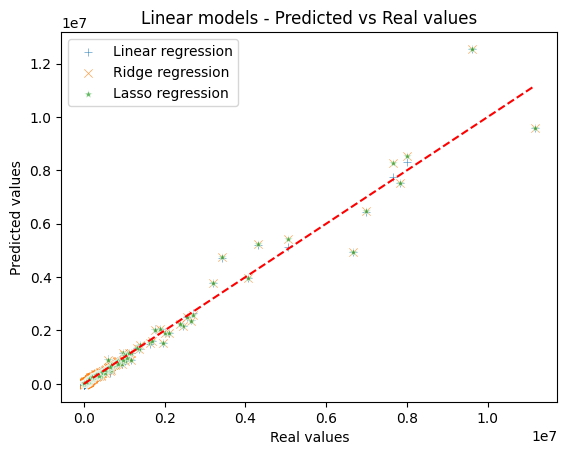
\includegraphics[width=\textwidth]{assets/images/linear-vs-ridge-vs-lasso-prediction.png}
         \caption{Prediction comparison}
     \end{subfigure}
     \caption{Result analysis for linear models}
\end{figure}
In term of metrics presented above, linear regression and ridge regression (+ cross validation) seem to be similar (linear regression is shorter to train). On the other hand, the importance of features is absolutely not the same depending on the model. This is quite unexpected, given that the data provided is the same and the features are normally relatively consistent with the problem set.
\\

It's curious that all points are predicted in the same way by all 3 models, even though they don't take the same features into account at all. The correctness of the models is therefore questionable.


\subsubsection{Interpretation of the results}
Let's analyse a bit the feature importance. We first can see that the two main features are related to localization of the train station, namely the total population living close to this train station and jobs in the attraction area. It is quite logical, but not what we expected. Indeed, it shows the dynamism of the attraction area in term of population (and activity), but we expected to have metrics such as the accomodations available for tourists, the size of the city...
\section{K-Nearest Neighbors}
In the same way as we have developed linear models, we have chosen to implement a model based on k nearest neighbors. We tuned the $k$ parameter to determine the optimal model. We also used the pipeline that was set up in the first examples to make the model as clear as possible and facilitate understanding.

\subsection{Model implementation}
\subsubsection{Implementation of a KNN model}
First, we set a simple knn model using the same pipeline we built in the last chapter. We then complexified the model to include cross-validation and parameter tuning to find the best hyper-parameters for our regression problem. We chose to \textbf{normalize} all the columns because of the properties of knn model (distance in space of features).

\subsubsection{Hyperparameters tuning}
As we did for the linear models, we chose to use \code{GridSearchCV} to tune the hyperparameter $k$ and find the fest model. By default (\href{https://scikit-learn.org/stable/modules/generated/sklearn.neighbors.KNeighborsClassifier.html}{scikit-learn documentation}), the model uses \textit{Minkowski} distance, but we chose to include distance function and how to weight neighbors' value.
\begin{lstlisting}
kf = KFold(n_splits=20, shuffle=True, random_state=42)
parameter = {
    'regressor__n_neighbors': np.arange(2, 30, 1),
    'regressor__metric': ['minkowski', 'euclidean', 'manhattan'],
    'regressor__weights': ['uniform', 'distance']
    }
...
knn_cv = GridSearchCV(knn, param_grid=parameter, cv=kf, verbose=1)
\end{lstlisting}
Then, we can extract the best hyperparameters from \code{regressor__n_neighbors} variable to train the tuned model.
\subsubsection{Check overfitting}
Learning curve (Figure~\ref{knn:learning-curve}) is a plot of the training and cross-validation error as a function of the training set size. It is a tool to find out how much we benefit from adding more training data and whether the estimator suffers more from a variance error or a bias error. We can use this to detect overfitting in the sense that a high training error and a low cross-validation error is a sign of overfitting.

\begin{figure}
    \centering
        \begin{subfigure}[b]{0.3\textwidth}
            \centering
            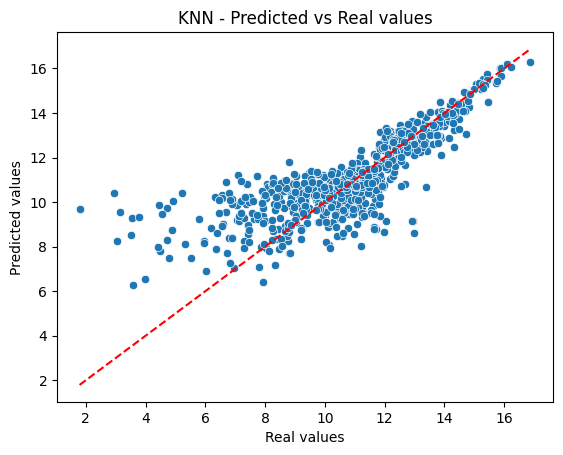
\includegraphics[width=\textwidth]{assets/images/knn-ypred-vs-ytest.png}
            \caption{$\hat{y}$ vs $y$ (log scale)}
            \label{knn:ypred-vs-yreal}
        \end{subfigure}
    \hfill
        \begin{subfigure}[b]{0.3\textwidth}
            \centering
            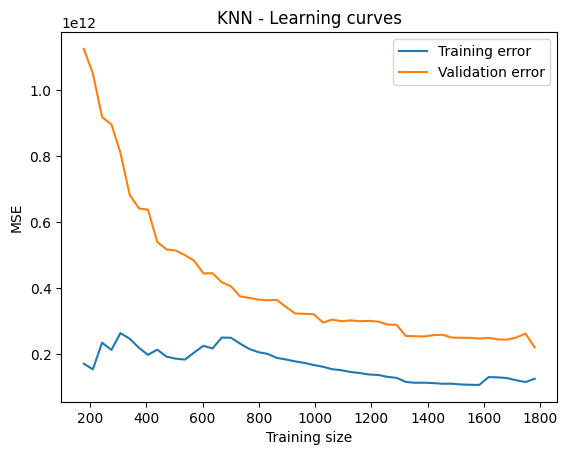
\includegraphics[width=\textwidth]{assets/images/knn-learning-curve.png}
            \caption{KNN learning curve}
            \label{knn:learning-curve}
        \end{subfigure}
    \hfill
        \begin{subfigure}[b]{0.3\textwidth}
            \centering
            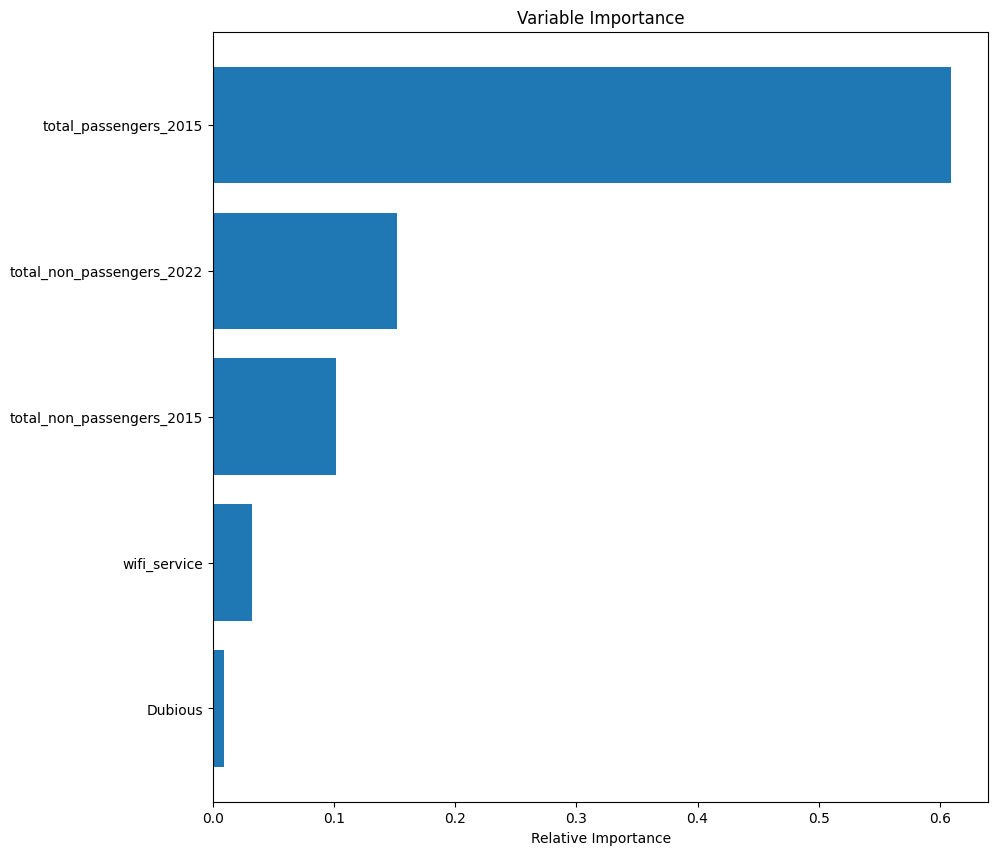
\includegraphics[width=\textwidth]{assets/images/knn-feature-importance.png}
            \caption{Feature importance}
            \label{knn:feature-importance}
        \end{subfigure}
    \caption{KNN metrics and performance analysis}
\end{figure}


\subsection{Results}
\subsubsection{Feature importance}
As the Lasso regularization, KNN models (tuned or raw) seems using quasi-only parameters related to train station (and not living area metrics) (see figure~\ref{knn:feature-importance}). As a consequence, we can ask if it it a good point to keep those very important features in the model. We conclude that, as the data is available, we should use it, like it would be in real problem solving.

\subsubsection{Performances}
Even if in linear scale, the KNN model seems to have good predictions, we can analyse $\hat{y}=f(y)$ (see figure \ref{knn:ypred-vs-yreal}). Indeed, we see that the model overestimates the traffic in train stations for low-traffic ones. This model is consequently adapted to our problem. Indeed, it is better to overestimate the traffic than just be flowed by too unpredicted people.

\begin{table}[h]
    \centering
    \begin{tabular}{ccccc}
        \toprule
        Model &  MSE &  MAE & MedianAE & $R^2$ Score \\
        \midrule
        Simple KNN model & 2.718e+11 & 140778 & 33152 & 0.834915\\
        KNN (best) & 2.176e+11 & 132651 & 30205 & 0.867865\\
        \bottomrule
    \end{tabular}
    \caption{Main metrics of KNN model}
\end{table}
We also see that the parameter tuning is useful, because we have $3,2$ points more for $R^2$ score (for instance).

\textbf{Observation:} As we don't have a lot of values for the high-traffic stations, the number of neighbors influence a lot the final prediction for those stations. Indeed, the points are really spread out, but knn model just compute the average of nearest points. This can lead to an unwanted approximation.
\section{Random forest}

\subsection{Data Preparation}
We started by loading the preprocessed dataset and defining the features and target variables for both regression and classification tasks. Categorical features were handled using one-hot encoding to convert them into a suitable format for model training. The dataset was then split into training and testing sets.

\subsection{Model Training and Evaluation}
We trained Random Forest models for both regression and classification tasks and compared their performance with Decision Tree and Gradient Boosting models.

\begin{table}[h]
    \centering
    \begin{tabular}{lllc}
        \toprule
        {} & Model & Metric & Score \\
        \midrule
        0 & Decision Tree Regression & MSE & 2.254280e+10 \\
        1 & Random Forest Regression & MSE & 1.069261e+10 \\
        2 & Gradient Boosting Regression & MSE & 2.286346e+09 \\
        3 & Decision Tree Classification & Accuracy & 9.573991e-01 \\
        4 & Random Forest Classification & Accuracy & 9.618834e-01 \\
        5 & Gradient Boosting Classification & Accuracy & 9.618834e-01 \\
        6 & Tuned Random Forest Regression & MSE & 9.932162e+09 \\
        7 & Tuned Random Forest Classification & Accuracy & 9.641256e-01 \\
        \bottomrule
    \end{tabular}
    \caption{Model Performance Metrics}
    \label{tab:model_performance}
\end{table}

\subsubsection{Regression}
The Random Forest Regression model was trained to predict the total number of passengers in 2022. We evaluated the model using the Mean Squared Error (MSE) metric.

\begin{figure}[H]
    \centering
    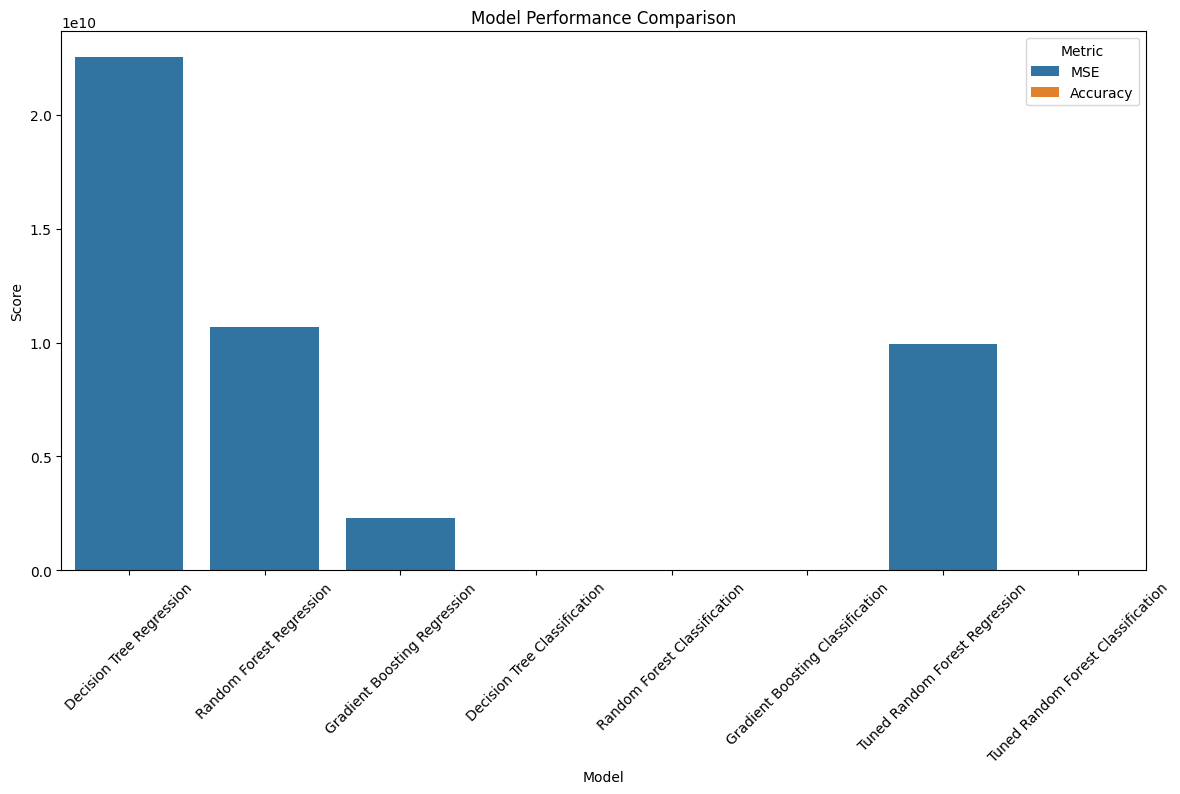
\includegraphics[width=0.7\textwidth]{assets/images/regression_performance.png}
    \caption{Model Performance Comparison for Regression}
    \label{fig:regression_performance}
\end{figure}

The Gradient Boosting Regression model outperformed the Decision Tree and Random Forest models, achieving the lowest MSE. The figure in \ref{fig:regression_performance} above shows the comparison of MSE across the models.


\begin{figure}[H]
    \centering
    \begin{subfigure}[H]{0.45\textwidth}
        \centering
        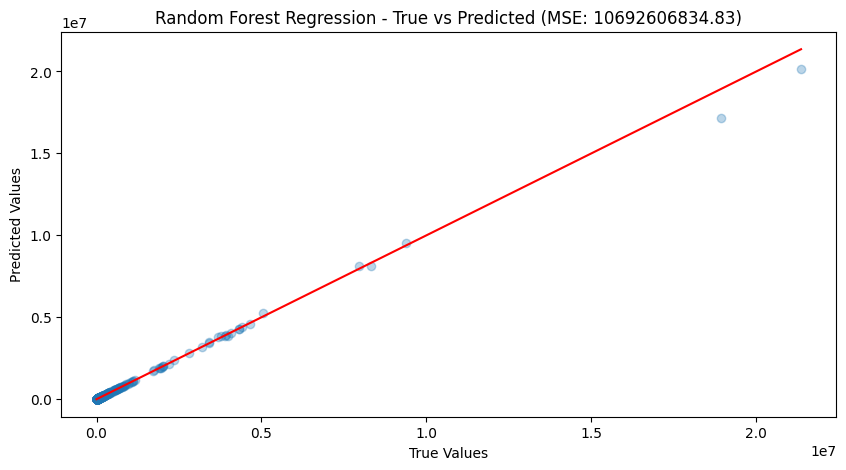
\includegraphics[width=\textwidth]{assets/images/random_forest_regression.png}
        \caption{Random Forest Regression - True vs Predicted Values}
        \label{fig:random_forest_regression}
    \end{subfigure}
    \hfill
    \begin{subfigure}[H]{0.45\textwidth}
        \centering
        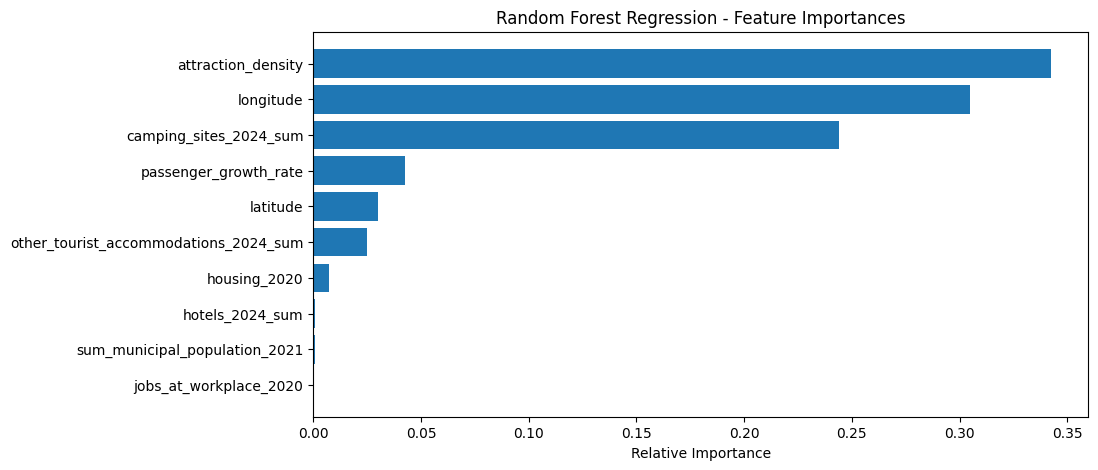
\includegraphics[width=\textwidth]{assets/images/feature_importance_random_forest.png}
        \caption{Feature Importance in Random Forest Regression}
        \label{fig:random_forest_feature_importance}
    \end{subfigure}
    \caption{Comparison of Random Forest Regression Results}
    \label{fig:random_forest_regression_comparison}
\end{figure}

Figure \ref{fig:random_forest_regression} shows the true vs predicted values for the Random Forest Regression model, indicating good alignment along the diagonal line. Figure \ref{fig:random_forest_feature_importance} highlights the most important features in the Random Forest Regression model, with \textit{attraction\_density} being the most significant.

\subsubsection{Classification}
The Random Forest Classification model was trained to predict whether a train station provides wifi service. We evaluated the model using the accuracy score metric.


\begin{figure}[H]
    \centering
    \begin{subfigure}[b]{0.3\textwidth}
        \centering
        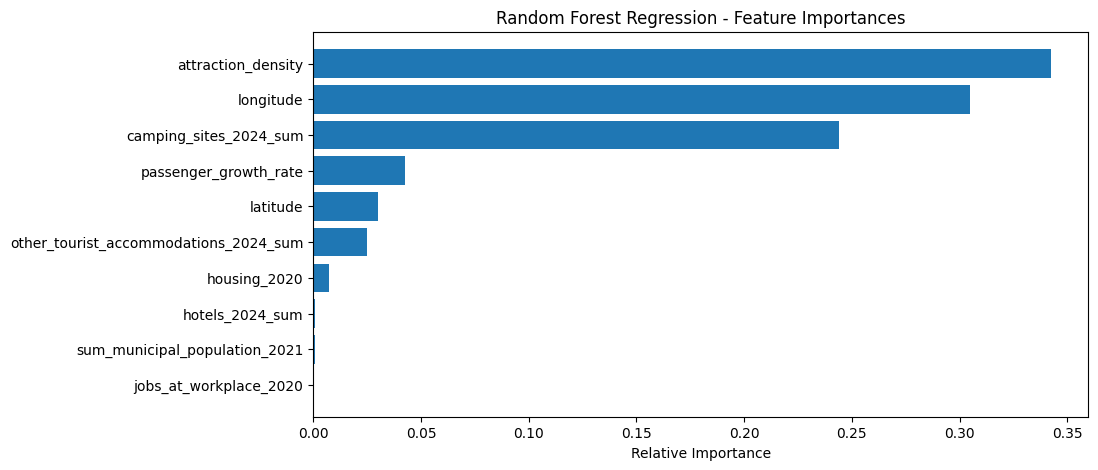
\includegraphics[width=\textwidth]{assets/images/random_forest_classification_feature_importance.png}
        \caption{Feature Importance for Random Forest Classification}
        \label{fig:random_forest_classification_feature_importance}
    \end{subfigure}
    \hfill
    \begin{subfigure}[b]{0.3\textwidth}
        \centering
        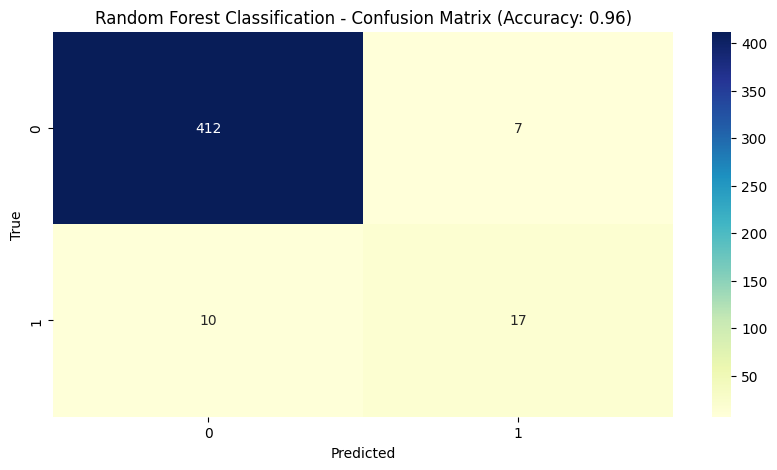
\includegraphics[width=\textwidth]{assets/images/random_forest_confusion_matrix.png}
        \caption{Confusion Matrix for Random Forest Classification}
        \label{fig:random_forest_classification_confusion}
    \end{subfigure}
    \hfill
    \begin{subfigure}[b]{0.3\textwidth}
        \centering
        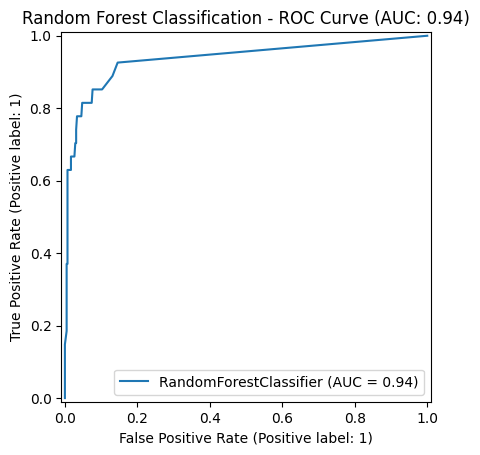
\includegraphics[width=0.75\textwidth]{assets/images/random_forest_ROC.png}
        \caption{ROC Curve for Random Forest Classification}
        \label{fig:random_forest_classification_ROC}
    \end{subfigure}
    \caption{Feature Importance, Confusion Matrix, and ROC for Random Forest Classification}
    \label{fig:classification_performance_and_confusion}
\end{figure}

The Random Forest Classification model achieved the highest accuracy compared to the Decision Tree and Gradient Boosting models. Figure \ref{fig:random_forest_classification_feature_importance} highlights the most important features used by the Random Forest Classification model. Figure \ref{fig:random_forest_classification_confusion} shows the confusion matrix for the Random Forest Classification model, indicating high accuracy. Figure \ref{fig:random_forest_classification_ROC} shows the ROC curve for the Random Forest Classification model, providing insights into the model's performance across different threshold settings. In the classification task, we faced class imbalance as the majority of the train stations do not provide wifi service. This was addressed using oversampling techniques to balance the classes and ensure that the model does not become biased towards the majority class.

\subsection{Hyperparameter Tuning}
To optimize the Random Forest models, we performed hyperparameter tuning using GridSearchCV. The best parameters for both regression and classification tasks were identified.

\subsection{Interpretation of Results}
The Gradient Boosting model showed the greatest performance in the regression task, while the Random Forest models demonstrated better performance in the classification task. Hyperparameter tuning further improved the performance of the Random Forest models, making them highly effective for both regression and classification.





\section{Support Vector Regression}
After the last lab, we decided to implement a SVM model for our regression problem.

\subsection{Model implementation}
\subsubsection{Simple linear model}
We build a simple model using \code{LinearSVR} model from scikit learn. The set up is the same than other models (pipeline, build and train the model, predict and analyse).
We get coherent and encouraging results for the two firsts models. First model was just a naive implementation of a LinearSVR model without parameter tuning, just using default values. For the second model, we did parameter tuning manually and build consequenly the best model among the tested ones.
\begin{figure}[h]
    \centering
    \begin{subfigure}[b]{0.35\textwidth}
         \centering
         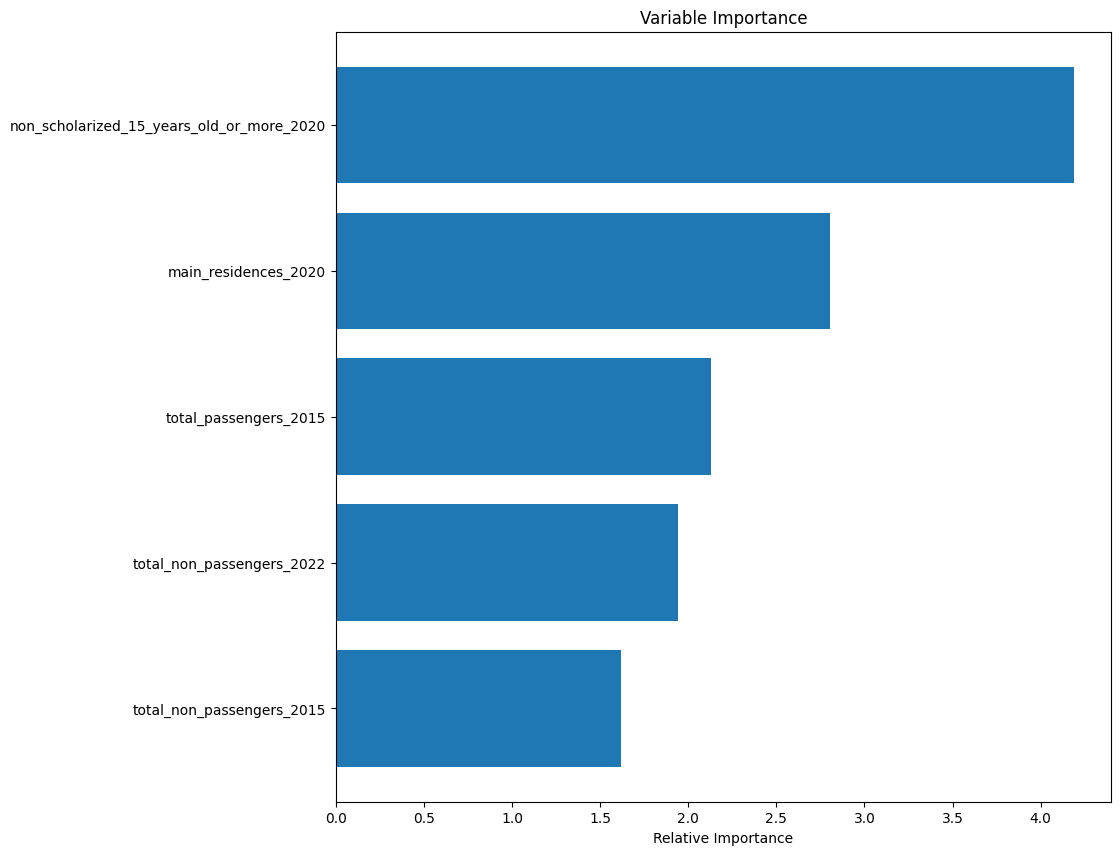
\includegraphics[width=\textwidth]{assets/images/linearsvr-tuning-feature-importance.png}
         \caption{LinearSVR: Feature importance}
     \end{subfigure}
     \hfill
     \begin{subfigure}[b]{0.35\textwidth}
         \centering
         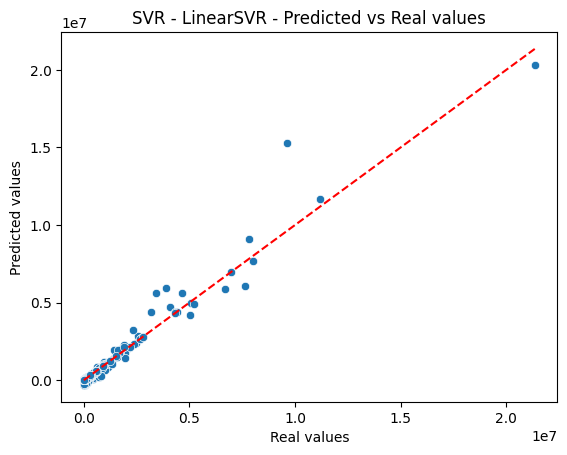
\includegraphics[width=\textwidth]{assets/images/linearsvr-tuning-ypred-vs-ytest.png}
         \caption{Prediction comparison}
     \end{subfigure}
     \caption{Result analysis for linear models}
\end{figure}

\begin{table}[h]
    \centering
    \begin{tabular}{ccccc}
        \toprule
        Model &  MSE &  MAE & MedianAE & $R^2$ Score \\
        \midrule
        LinearSVR tuned manually & 7.801625e+10 & 62390.014597 & 9074.516478 & 0.952629\\
        \bottomrule
    \end{tabular}
    \caption{Main metrics to compare LinearSVR model}
\end{table}

\subsection{Kernel and other parameters tuning}
When trying to train the model in different other kernels, we faced a lot of issues. We think it is caused by our dataset. Indeed, the training time was infinite (we let the model train for 12 hours without result). We also got completely broken results as you can see in the \href{https://github.com/pierre-jezegou/fib-ml-project/blob/main/models/svm.ipynb}{\code{models/svm.ipynb}}
\chapter{Model comparison}
\section{Metrics used to compare the models}
Mean Squared Error (MSE) measures the average of the squares of the errors or deviations, indicating the model's risk corresponding to the expected value of the squared error loss. Mean Absolute Error (MAE) represents the average absolute difference between predicted and actual values, providing a clear indication of the average error magnitude. Median Absolute Error (MedianAE) provides the median of all absolute differences between predicted and actual values, being less sensitive to outliers compared to MAE. The R² Score indicates how well the model's predictions match the actual data, with a higher R² score signifying better model performance. For classification tasks, Accuracy measures the proportion of true results (both true positives and true negatives) among the total number of cases examined. The Confusion Matrix helps in understanding the performance of a classification model by showing the actual versus predicted classifications.

\section{Comparison}
We implemented and evaluated several models, including Linear Regression, Ridge Regression, Lasso Regression, K-Nearest Neighbors (KNN), Random Forest, Gradient Boosting, and Support Vector Regression (SVR). Below is a summary of the results and insights for each model based on the aforementioned metrics.
{\small
\begin{itemize}
    \item For linear models, Linear Regression achieved an MSE of 4.232e+10, an MAE of 54041, and an R² score of 0.968842. Ridge Regression had an MSE of 4.242e+10, an MAE of 51118, and an R² score of 0.968726. Lasso Regression resulted in an MSE of 4.366e+10, an MAE of 52531, and an R² score of 0.967857.
    \item For the K-Nearest Neighbors (KNN) model, the simple KNN model had an MSE of 2.718e+11, an MAE of 140778, and an R² score of 0.834915. The tuned KNN model improved to an MSE of 2.176e+11, an MAE of 132651, and an R² score of 0.867865.
    \item The Random Forest model for regression had an MSE of 1.069261e+10, an MAE of 62390.014597, and an R² score of 0.952629. For classification, it achieved an accuracy of 0.9618834.
    \item Gradient Boosting for regression achieved the best performance with an MSE of 2.286346e+09 and an R² score of 0.968842. For classification, it matched the Random Forest model with an accuracy of 0.9618834.
    \item Support Vector Regression (SVR) with the LinearSVR model resulted in an MSE of 7.801625e+10, an MAE of 62390.014597, and an R² score of 0.952629.
\end{itemize}
}


\section{Best model for our problem}
Considering both the regression and classification tasks, the Gradient Boosting Regression model is the best choice for predicting the total number of passengers, given its lowest MSE (2.286346e+09) and high R² score. For example, Gradient Boosting Regression outperformed Random Forest Regression (MSE: 1.069261e+10) and Linear Regression (MSE: 4.232e+10), showing its superiority in capturing complex patterns in the data.

For classification tasks, such as predicting whether a train station provides WiFi service, the Random Forest Classification model is the most effective due to its higher accuracy (0.9618834). The confusion matrix for Random Forest Classification showed a high number of correctly classified instances, and the ROC curve indicated strong performance across different threshold settings.
\chapter{Conclusion}

\section{Scientific and Personal Reflections}
This project was a great learning experience in the field of machine learning. We explored various techniques and worked with real-world data, which was both challenging and rewarding. We compared and implemented different methods, and used advanced tools like GridSearchCV. Online resources, especially the scikit-learn documentation, were very helpful.

Understanding the dataset before starting was difficult. Our dataset had limitations that made it hard to apply everything we learned in lectures, showing the gap between theory and practice.

\section{Possible Extensions and Known Limitations}
For future work, we could try new models and add more data when it becomes available, possibly next year. We could also use Generative Adversarial Networks (GANs) to create synthetic data, which might improve our models.

\section{Challenges Faced}
Throughout the project, we faced several challenges:

\begin{itemize}
    \item There were a lot of features to handle, which was overwhelming.
    \item The models showed a lot of differences in prediction accuracy and feature importance, making it hard to choose the best one.
    \item The dataset was not evenly distributed across the country, with too much data from Paris train stations, causing bias.
    \item Working with real-world data is complex. We had to understand the data well without changing it too much to avoid influencing the models.
    \item Dealing with non-optimized, real data was a constant challenge that required ongoing problem-solving. This project showed us the importance of being flexible and persistent when working with complex data.
\end{itemize}

In summary, this project gave us valuable insights into the practical side of machine learning. It reinforced our theoretical knowledge and highlighted the complexities and challenges of working with real-world data.
\end{document}